\documentclass{beamer}

\usepackage[lined, vlined]{algorithm2e}
\usepackage{amsmath, amssymb, amsfonts}
\usepackage{caption}
\usepackage{color}
\usepackage{graphicx}
\usepackage{multirow}
\usepackage{pgfplots}
\usepackage{tikz}

\usetheme{CambridgeUS}

\newcommand{\Field}{\mathbb{F}}
\newcommand{\FField}[1]{\Field_{#1}}
\newcommand{\Ideal}[1]{\langle #1 \rangle}
\newcommand{\LT}[1]{\mathsf{LT}(#1)}
\newcommand{\LM}[1]{\mathsf{LM}(#1)}
\newcommand{\LC}[1]{\mathsf{LC}(#1)}
\newcommand{\Tail}[1]{\mathsf{Tail}(#1)}
\newcommand{\Term}[1]{\mathsf{Term}(#1)}
\newcommand{\Mono}[1]{\mathsf{Mono}(#1)}
\newcommand{\term}{\mathfrak{t}}
\newcommand{\mono}{\mathfrak{m}}
\newcommand{\coef}{\mathfrak{c}}
\newcommand{\mpolyring}[3]{#1[#2_{1}, \ldots, #2_{#3}]}
\newcommand{\LCM}[2]{\mathsf{LCM}(#1, #2)}
\newcommand{\LCMLM}[2]{\LCM{\LM{#1}}{\LM{#2}}}
\newcommand{\Spoly}[2]{\mathsf{Spoly}(#1, #2)}
\newcommand{\Grobner}{Gr\"{o}bner }
\newcommand{\ZZ}{\mathbb{Z}}

\newcommand{\Alg}[2]{\textsc{#1}(#2)}
\newcommand{\FullReduce}[1]{\Alg{FullReduce}{#1}}
\newcommand{\MulFullReduce}[1]{\Alg{MulFullReduce}{#1}}
\newcommand{\GetReductor}[1]{\Alg{GetReductor}{#1}}
\newcommand{\SelectReductor}[1]{\Alg{SelectReductor}{#1}}
\newcommand{\UpdateReduce}[1]{\Alg{UpdateReduce}{#1}}

\newtheorem{question}{Question}
\newtheorem{link}{}

\title{M4GB: An Efficient \Grobner Basis Algorithm} \author{Rusydi
  H. Makarim\inst{1, 2} \and Marc Stevens\inst{2}}
\institute{\inst{1}Mathematics Institute, University Leiden \and
  \inst{2}Cryptology Group, Centrum Wiskunde en Informatica (CWI)}

\date{ALGANT-DOC Meeting, 15th May 2017}

\AtBeginSection[]
{
  \begin{frame}{Table of Contents}
    \tableofcontents[currentsection]
  \end{frame}  
}


\begin{document}

\begin{frame}
  \titlepage
\end{frame}

\begin{frame}
  \tableofcontents
\end{frame}

\begin{section}{Introduction}
  
  \begin{frame}{Problem}

    \begin{itemize}
    \item $\Field$ - A Field
    \item $n$ - number of variables
    \item $m$ - number of equations
    \end{itemize}

    \pause
    
    \begin{problem}<2->[Multivariate Quadratic(MQ) problem]

      \begin{itemize}
      \item<3-> Given : $f_1, \ldots, f_m \in \mpolyring{\Field}{x}{n}$, $\deg(f_i) = 2$
      \item<4-> Problem : Find a $(v_1, \ldots, v_n) \in \Field^n$ such that
        \begin{align*}
        f_1(v_1, \ldots, v_n) &= 0\\
        &\vdots\\
          f_m(v_1, \ldots, v_n) &= 0
        \end{align*}
      \end{itemize}
    \end{problem}
  \end{frame}

  \begin{frame}{Why MQ Problem ?}
    \begin{itemize}
    \item<1-> MQ-problem is NP-complete
    \item<2-> Candidate for post-quantum public-key and digital-signature scheme
    \item<3-> Need to understand its practical difficulty (How ?)
    \end{itemize}

    \begin{block}<4->{Open Public Challenge - MQChallenge}
      \begin{itemize}
      \item Initiated at 2015
      \item Random and dense system
      \item Various parameters
      \end{itemize}
    \end{block}
  \end{frame}

  \begin{frame}{MQ Challenge Types}
    \begin{table}
      \center
      \begin{tabular}{|c|c|c|c|}
        \cline{2-4}
        \multicolumn{1}{c|}{} & $\FField{2}$ & $\FField{2^8}$ & $\FField{31}$\\
        \hline
        \multirow{2}{*}{$m = 2n$} & \onslide<2->{\Large{I}} &  \onslide<2->{\Large{II}} & \onslide<2->{\Large{III}} \\
        \cline{2-4}
        & \onslide<3->{$n \geq 55$} & \onslide<3->{$n \geq 35$} & \onslide<3->{$n \geq 34$}\\
        \hline
        \hline
        \multirow{2}{*}{$m \approx 2/3 n$} & \onslide<4->{\Large{IV}} & \onslide<4->{\Large{V}} & \onslide<4->{\Large{VI}} \\
        \cline{2-4}
        & \onslide<5->{$m \geq 55$} & \onslide<5->{$m \geq 16$} & \onslide<5->{$m \geq 16$}\\
        \hline
      \end{tabular}
    \end{table}
    \begin{block}<6->{Parameter Choice}
      Require at least \alert{one month}
      for Magma 2.19-9 to solve using \alert{Four 6-cores Intel(R)
      Xeon(R) CPU E5-4617 @ 2.9GHz} and \alert{1TB of RAM}.
    \end{block}
    \onslide<7->{\center{\url{https://www.mqchallenge.org}}}
  \end{frame}

  \begin{frame}{Solving MQ-problem}
    \begin{itemize}
    \item<1-> Linearization
    \item<2-> Extended Linearization (XL)
    \end{itemize}
    \begin{block}<3->{This talk}
      \center{\LARGE{\Grobner basis}}
    \end{block}
  \end{frame}
\end{section}

\begin{section}{\Grobner Basis}
  % Monomial Ordering
  \begin{frame}{Ordering Monomial in $\mpolyring{\Field}{x}{n}$}
    \begin{definition}[Monomial Ordering]
      $>$ is a monomial ordering if
      \begin{enumerate}
      \item<2-> Total (or linear) ordering on $\ZZ_{\geq 0}^{n}$
      \item<3-> Let $\alpha, \beta, \gamma \in \ZZ_{\geq 0}^n$ and $x = (x_1, \ldots, x_n)$
        $$
        x^{\alpha} > x^{\beta} \Rightarrow x^{\gamma} x^{\alpha} > x^{\gamma} x^{\beta}
        $$
        \item<4-> $>$ is a well-ordering on $\ZZ_{\geq 0}^n$
      \end{enumerate}
    \end{definition}
  \end{frame}

  \begin{frame}{Monomial Ordering : Examples}
    \begin{block}<1->{Lexicographic}
      \begin{center}
        $x^{\alpha} >_{\mathrm{lex}} x^{\beta} \Leftrightarrow$ the leftmost nonzero entry of $\alpha - \beta$ is positive
      \end{center}
    \end{block}

    \begin{block}<2->{Degree-Reverse Lexicographic (degrevlex)}
      $x^{\alpha} >_{\mathrm{degrevlex}} x^{\beta} \Leftrightarrow$
      \begin{itemize}
      \item<3-> $\sum_{i} \alpha_i > \sum_{i} \beta_i$ \quad OR
      \item<4-> $\sum_{i} \alpha_i = \sum_{i} \beta_i$ and the rightmost nonzero entry of $\alpha - \beta$ is negative
      \end{itemize}
    \end{block}
  \end{frame}

  \begin{frame}{Notations}
    $\mpolyring{\Field}{x}{n}$ together with $>$

    \begin{block}<2->{Notations}
      $f \in \mpolyring{\Field}{x}{n}$, $f \neq 0$
      \begin{itemize}
      \item<3-> $\LM{f}$ (the largest monomial of $f$ w.r.t $>$)
      \item<4-> $\LC{f}$ (the coefficient correspond to $\LM{f}$)
      \item<5-> $\LT{f} = \LC{f} \cdot \LM{f}$
      \item<6-> $\Tail{f} = f - \LT{f}$
      \item<7-> $\Term{f}$, $\Mono{f}$
      \end{itemize}
    \end{block}
    \onslide<8->
    {
    $$
    F \subseteq \mpolyring{\Field}{x}{n}
    \begin{cases}
      \Tail{F} = \cup_{f \in F} \{ \Tail{f} \}\\
      \Term{F} = \cup_{f \in F} \Term{f}\\
      \Mono{F} = \cup_{f \in F} \Mono{f}
    \end{cases}
    $$
    }
    % \begin{block}{Example}
    %   $f = \alert<4> {\alert<3>{-15} \alert<2>{x^2}} + \alert<5>{8xy -
    %     13z^2 - 4x + 11z} \in \FField{31}[x, y, z]$

    %   $\LM{f} = x^2$, $\LC{f} = -15$, $\LT{f} = -15x^2$
    % \end{block}
  \end{frame}

  \begin{frame}{\Grobner Basis : Definition}
    \begin{definition}
      \onslide<2->{$I \neq \{ 0 \}$ be an ideal of $\mpolyring{\Field}{x}{n}$}\\
      \onslide<3->{$G \subseteq I$, $|G| < \infty$ that generates $I$ is a \Grobner basis of $I$ if,}

      \onslide<4->{\center{for any $f \in I$, $\exists g \in G$ s.t. $\LT{g} \mid \LT{f}$}}
    \end{definition}
  \end{frame}
  
  \begin{frame}{\Grobner Basis and Solving System of Equations}
    \begin{block}<2->{Lexicographic Ordering}
      \begin{align*}
      &g_1(x_1), \ldots,\\
      &g_2(x_1, x_2), \ldots, g_{k_1}(x_1, x_2)\\
      &g_{k_1 + 1}(x_1, x_2, x_3), \ldots,\\
      &g_{k_n}(x_1, \ldots, x_n)
      \end{align*}
    \end{block}

    \begin{block}<3->{Unique Solution in the Base Field}
      \begin{align*}
        g_1 = x_1 &+ c_1,\\
            &\vdots\\
        g_n = x_n &+ c_n
      \end{align*}
    \end{block}
  \end{frame}

  \begin{frame}
    \begin{question}<2->
      Given $f_1, \ldots, f_m \in \mpolyring{\Field}{x}{n}$, how to compute the \Grobner basis $G$ of $\Ideal{f_1, \ldots, f_m}$ ?
    \end{question}

    \begin{block}<3->{How to obtain new element in the ideal ?}
      \begin{enumerate}
      \item<4-> Generate polynomials of higher degree
      \item<5-> Division algorithm in $\mpolyring{\Field}{x}{n}$ (computing remainder)
      \end{enumerate}
    \end{block}
  \end{frame}

  \begin{frame}{Generate higher degree polynomial : S-Polynomial}
    \begin{itemize}
    \item<2-> $f, g \in \mpolyring{\Field}{x}{n}$ with $f \neq 0, g \neq 0$
    \item<3-> $x^{\gamma} = \LCMLM{f}{g}$
    \end{itemize}
    \begin{definition}<4->
      $$
      \Spoly{f}{g} = \dfrac{x^{\gamma}}{\LT{f}} \cdot f -
      \dfrac{x^{\gamma}}{\LT{g}} \cdot g.
      $$
    \end{definition}
  \end{frame}

  \begin{frame}{Division Algorithm in $\mpolyring{\Field}{x}{n}$ : Example}
    \begin{table}
      \begin{tabular}{r|ll}
        \multicolumn{1}{c}{} & $\onslide<2->{xy} \onslide<9->{- z} \onslide<12->{+ 1}$ & \hspace{10mm} \onslide<5->{$r$}\\
        \cline{2-2}
        $xy + z$ & $x^2 y^2 + z^4 + xy$ \\
        \multicolumn{1}{c}{} & \onslide<3->{$x^2y^2 + xyz$} &\\
        \cline{2-2}
        \multicolumn{1}{c}{} & \onslide<4->{$z^4 - xyz + xy$} & \hspace{10mm}\onslide<6->{$z^4$}\\
        \multicolumn{1}{c}{} & \onslide<7->{$z^4$} & \\
        \cline{2-2}
        \multicolumn{1}{c}{} & \onslide<8->{$-xyz + xy$} & \\
        \multicolumn{1}{c}{} & \onslide<10->{$-xyz - z^2$} & \\
        \cline{2-2}
        \multicolumn{1}{c}{} & \onslide<11->{$xy + z^2$} & \\
        \multicolumn{1}{c}{} & \onslide<13->{$xy + z$} & \\
        \cline{2-2}
        \multicolumn{1}{c}{} & \onslide<14->{$z^2 - z$} & \hspace{10mm}\onslide<15->{$z^4 + z^2$}\\
        \multicolumn{1}{c}{} & \onslide<16->{$z^2$} & \\
        \cline{2-2}
        \multicolumn{1}{c}{} & \onslide<17->{$-z$} & \hspace{10mm}\onslide<18->{$z^4 + z^2 - z$}\\
        \multicolumn{1}{c}{} & \onslide<19->{$-z$} & \\
        \cline{2-2}
        \multicolumn{1}{c}{} & \onslide<20->{$0$} & \\
      \end{tabular}
    \end{table}
  \end{frame}

  \begin{frame}{Division Algorithm / Polynomial Reduction}

    $G = (g_1, \ldots, g_t) \subseteq \mpolyring{\Field}{x}{n}$

    \begin{theorem}<2->[Division Algorithm]
      Every $f \in \mpolyring{\Field}{x}{n}$ can be written as
      $$
      f = q_1 g_1 + \ldots + q_t g_t + r
      $$
      and
      $$
      r =
      \begin{cases}
        0 \\
        \text{none of terms of $r$ is divisible by any of $\LT{g_i}$}
        \end{cases}
      $$
    \end{theorem}

    \onslide<3->{\center{$r \leftarrow \textsc{FullReduce}(f, G)$}}
  \end{frame}


  \begin{frame}{Buchberger's Algorithm}
    \begin{algorithm}[H]
      \KwIn{A finite ordered subset
        $F \subseteq \mpolyring{\Field}{x}{n}$} \KwResult{A \Grobner
        basis $G$ such that $\Ideal{G} = \Ideal{F}$}

      $G \leftarrow F$\\
      \Repeat{$G = G'$}
      {
        $G' \leftarrow G$\\
        \ForAll{ $(p, q) \in G' \times G'$, $p \neq q$}
        {
          $r \leftarrow \FullReduce{\Spoly{p}{q}, G'}$\\
          \If{$r \neq 0$}
          {
            $G \leftarrow G \cup \{ r \}$
          }
        }
      }
      \Return{$G$}
    \end{algorithm}

    % \begin{algorithm}[H]
    %   \KwIn{A finite ordered subset
    %     $F \subseteq \mpolyring{\Field}{x}{n}$} \KwResult{A \Grobner
    %     basis $G$ such that $\Ideal{G} = \Ideal{F}$}

    %   $P \leftarrow \{ \{p, q \} : \forall p, q \in F\ \mathbf{and}\ p \neq q \}$\\
    %   $G \leftarrow F$\\

    %   \While{$P \neq \{ \}$} {
    %     $\{ p, q \} \leftarrow \textsc{Select}(P)$\\
    %     $P \leftarrow P \setminus \{ \{ p, q \} \}$\\
    %     $r \leftarrow \textsc{FullReduce}(\Spoly{p}{q}, G)$\\
    %     \If{$r \neq 0$} {
    %       $P \leftarrow P \cup \{ \{r, g \} : \forall g \in G\}$\\
    %       $G \leftarrow G \cup \{ r \}$ } } \Return{$G$}
    % \end{algorithm}
  \end{frame}
\end{section}


\begin{section}{M4GB Algorithm}
  \begin{frame}
    \begin{itemize}
    \item<1-> \Grobner bases algorithms follows the same principle
    \item<2-> Differs in reduction techniques
    \end{itemize}
  \end{frame}

  \begin{frame}{Example : Standard Reduction vs M4GB Reduction}
    \begin{normalsize}
      $\FField{2}[x_1, x_2, x_3, x_4]$ with \emph{degrevlex} ordering
    \end{normalsize}
    \vspace{2mm}
    \begin{columns}[T]
      \begin{column}<2->[T]{.50\textwidth}
        \begin{small}
          $f = \textcolor<4>{red}{x_1^2 x_2^3} + x_1 x_2^3 x_4 + x_1 x_3^3 + x_1^3 x_4 + x_2 x_3^2 + x_4^2$\\
          \onslide<5->{$f = f - g_1 = \textcolor<6,11>{red}{x_1 x_2^3 x_4} + x_1^3 x_4 + x_2 x_3^2$}
          \onslide<12->{$f = f - g_4 = x_1^3 x_4 + x_2 x_3^2 + 1$}
        \end{small}
      \end{column}
      \vrule{}
      \begin{column}<3->[T]{.50\textwidth}
        \begin{small}
          $G = \{ g_1, g_2, g_3 \onslide<10->{, \textcolor<10>{orange}{g_4} } \}$\\
          \vspace{2mm}
          $g_1 = \textcolor<4>{red}{x_1^2 x_2^3} + x_1 x_3^3 + x_4^2$\\
          \vspace{1mm}
          $g_2 = \textcolor<6>{orange}{x_2^3 x_4} + x_2 x_3 + x_3 + 1$\\
          \vspace{1mm}
          $g_3 = \textcolor<9>{red}{x_1 x_2 x_3} + x_1 x_3$\\
          \vspace{1mm}
          \onslide<10->{$ \textcolor<10>{orange}{g_4} = x_1g_2 - g_3 = \textcolor<11>{red}{x_1 x_2^3 x_4} + 1$\\}
          \vspace{5mm}
          \onslide<7->{$x_1 g_2 = x_1 x_2^3 x_4 + \textcolor<8>{orange}{\textcolor<9>{red}{x_1 x_2 x_3} + x_1 x_3 + x_1}$\\}
        \end{small}
      \end{column}
    \end{columns}
    \center{\onslide<13->{$r = x_1^3 x_4 + x_2 x_3^2 + 1$}}
  \end{frame}

  \begin{frame}
    \begin{block}{M4GB Main Strategy}
      Maintain tail-reduced polynomials
    \end{block}
  \end{frame}

  \begin{frame}{M4GB Reduction}
    \vspace{-1.5cm}
    \begin{columns}[T]
      \begin{column}[T]{.50\textwidth}
        \begin{scriptsize}
          \center{$\MulFullReduce{G, u, f}$}\\
          \vspace{0.3cm}
          \begin{algorithm}[H]
          $r \leftarrow 0$\\
          \ForAll{$t \in \Term{f}$} {
            $t' \leftarrow u \cdot t$\\
            \If{$\exists g \in G : \LT{g} \mid t'$}
            {
              $(G, g) \leftarrow \GetReductor{G, t'}$\\
              $r \leftarrow r - (t' / \LT{g}) \cdot \Tail{g}$
            }
            \Else
            {
              $r \leftarrow r + t'$
            }
          }
          \Return{$(G, r)$}
          \end{algorithm}
        \end{scriptsize}
      \end{column}
      \begin{column}<2->[T]{.50\textwidth}
        \begin{scriptsize}
          \center{$\GetReductor{G, t}$}\\
          \vspace{0.3cm}
          \begin{algorithm}[H]
            \If{$\exists g \in G : \LM{g} = \LM{t}$}
            {
              \Return{$(G, g)$}
            }
            $h \leftarrow \SelectReductor{G, t}$\\
            $(G, h) \leftarrow \MulFullReduce{G, t / \LT{h}, \Tail{h}}$\\
            $g \leftarrow t + h$\\
            \Return{$(G \cup \{ g\}, g)$}
          \end{algorithm}
        \end{scriptsize}
      \end{column}
    \end{columns}
  \end{frame}

  \begin{frame}
    \center{$\UpdateReduce{G, f}$}
    \begin{algorithm}[H]
      \begin{footnotesize}
      $H \leftarrow \{ \LC{f}^{-1} \cdot f \}$\\
      $Q \leftarrow \Mono{ \Tail{G \cup H} } \setminus \LM{H}$\\
      \vspace{3mm}
      \While{$\exists u \in Q : \LM{f} \mid u$}
      {
        $u \leftarrow \max \{ \mono \in Q : \LM{f} \mid \mono \}$\\
        $(G, h) \leftarrow \MulFullReduce{G, u / \LT{f}, \Tail{f}}$\\
        $H \leftarrow H \cup \{ u + h\}$\\
        $Q \leftarrow \Mono{ \Tail{G \cup H} } \setminus \LM{H}$
      }
      \vspace{3mm}
      \While{$H \neq \{ \} $}
      {
        Select $h \in H$ such that $\LM{h} = \min \LM{H}$\\
        $H \leftarrow H \setminus \{ h \}$\\
        $H \leftarrow \{ g - ch : g \in H, c$ is a coefficient of $\LM{h}$ in $\Tail{g} \}$\\
        $G \leftarrow \{ g - ch : g \in G, c$ is a coefficient of $\LM{h}$ in $\Tail{g} \}$\\
        $G \leftarrow G \cup \{ h \}$\\
      }
      \end{footnotesize}
    \end{algorithm}
  \end{frame}

\end{section}


\begin{section}{Performance Comparison}
  \begin{frame}
    \begin{itemize}
    \item<1-> Implemented using \texttt{C++11}
    \item<2-> Comparison with existing implementations
      \begin{enumerate}
      \item FGb C Interface - Implementation by Jean Charles
        Faugere\footnote<2->{Available at
          \url{http://www-polsys.lip6.fr/~jcf/FGb/C/index.html}}
      \item Magma v2.20-6
      \item OpenF4 v1.0.1 - Open source implementation by Coladon,
        Vitse and Joux\footnote<2->{Available at
          \url{https://github.com/nauotit/openf4}}.
      \end{enumerate}

    \item<3-> Test cases
      \begin{enumerate}
      \item Dense polynomials with coefficients in $\FField{31}$
      \item $m = 2n$ and $m = n + 1$.
      \end{enumerate}
      
     
    \end{itemize}
    
  \end{frame}

  \begin{frame}{Benchmark for $m = 2n$}
    \vspace{-3mm}
    \begin{scriptsize}
      \begin{table}
        \begin{tabular}[h]{|c|c|c|c|c|c|}
          \hline
          \multicolumn{2}{|c|}{} &\multicolumn{4}{c|}{Total CPU time (sec)}\\
          \hline
          $n$ & $m$   & M4GB    & OpenF4  & Magma    & FGb      \\
          \hline
          $20$ & $40$ & $57$    & $206$   & $232$    & $470$    \\
          $21$ & $42$ & $170$   & $472$   & $500$    & $1002$   \\
          $22$ & $44$ & $424$   & $1145$  & $1617$   & $3118$   \\
          $23$ & $46$ & $1060$  & $2274$  & $3185$   & $6849$   \\
          $24$ & $48$ & $2556$  & $10293$ & $31168$  & $64700$  \\
          $25$ & $50$ & $5575$  & -       & $77679$  & $151653$ \\
          $26$ & $52$ & $15517$ & -       & $183629$ & $360055$ \\
          $27$ & $54$ & $46548$ & -       & $409452$ & $767543$ \\
          \hline\hline
          \multicolumn{2}{|c|}{} & \multicolumn{4}{c|}{Memory (MB)} \\
          \hline
          $n$ & $m$ & M4GB & FGb    & Magma   & OpenF4   \\
          \hline
          20 & 40 & $73$   & $112$  & $362$   & $4240$   \\
          21 & 42 & $121$  & $165$  & $577$   & $6640$   \\
          22 & 44 & $226$  & $525$  & $859$   & $14368$  \\
          23 & 46 & $395$  & $918$  & $1324$  & $26135$  \\
          24 & 48 & $663$  & $1561$ & $8873$  & $161945$ \\
          25 & 50 & $1471$ & $2765$ & $19719$ & -        \\
          26 & 52 & $3328$ & $4607$ & $25197$ & -        \\
          27 & 54 & $6799$ & $8180$ & $39845$ & -        \\
          \hline
        \end{tabular}
      \end{table}
    \end{scriptsize}
  \end{frame}

  
  \begin{frame}{Graph for $m = 2n$}
    \vspace{-10mm}
    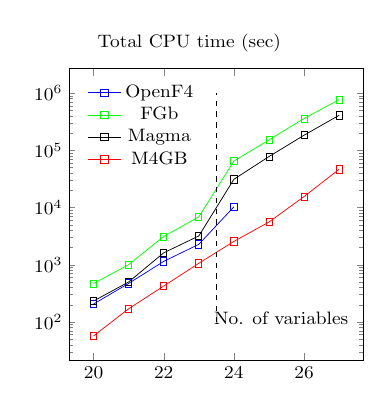
\begin{tikzpicture}[xscale=0.7, yscale=0.65]
      \begin{semilogyaxis}
		[ title={Total CPU time (sec)}, xlabel={No. of variables},
        % ylabel={(sec)},
        x label style={at={(axis description
            cs:.9,0.1)},anchor=south},
        % y label style={at={(axis description
        % cs:0.15,.43)},anchor=north},
        legend pos=north west, legend style={draw=none,fill=none},
        grid style=dashed,
        % scale=0.7 ymin=10,ymax=1000000 xmin=20,xmax=27,
        xscale=0.78 ]
		
		\addplot[color=blue, mark=square]
        coordinates{(20,206)(21,472)(22,1145)(23,2274)(24,10293)};
		
		\addplot[color=green,mark=square]
        coordinates{(20,470)(21,1002)(22,3118)(23,6849)(24,64700)(25,151653)(26,360055)(27,767543)%(28,1578995)
        };
		
		\addplot[color=black,mark=square]
        coordinates{(20,232.16)(21,500.26)(22,1616.73)(23,3184.81)(24,31167.61)(25,77678.58)(26,183628.74)(27,409451.87)%(28,838817.93)
        };
		
		\addplot[color=red,mark=square]
        coordinates{(20,57)(21,170)(22,424)(23,1060)(24,2556)(25,5575)(26,15517)(27,46548)%(28,146204)
        };
        
        \addplot +[mark=none,color=black, style=dashed] coordinates
        {(23.5, 100) (23.5, 1000000)};
        % \node[anchor={north west},rotate=270] at (axis cs:
        % 23.5,1000000) { DoR 5 };
        % \node[anchor={south west},rotate=270] at (axis cs:
        % 23.5,1000000) { DoR 6 };
        
        \legend{OpenF4, FGb, Magma, M4GB}
      \end{semilogyaxis}
      % \draw
    \end{tikzpicture}
    \hspace{10mm}
    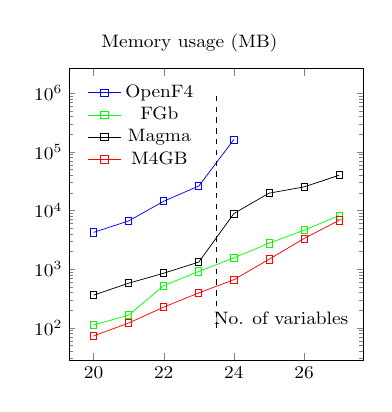
\begin{tikzpicture}[xscale=0.7, yscale=0.65]
      \begin{semilogyaxis}
		[ title={Memory usage (MB)}, xlabel={No. of variables},
        % ylabel={Memory (MB)},
        x label style={at={(axis description
            cs:.9,0.1)},anchor=south},
        % y label style={at={(axis description
        % cs:0.2,.5)},anchor=north},
        legend pos=north west, legend style={draw=none,fill=none},
        grid style=dashed, xscale=0.78 ]
		
		\addplot[color=blue, mark=square]
        coordinates{(20,4240)(21,6640)(22,14368)(23,26135)(24,161945)};
		
		\addplot[color=green,mark=square]
        coordinates{(20,112)(21,165)(22,525)(23,918)(24,1561)(25,2765)(26,4607)(27,8180)%(28,12982)
        };
		
		\addplot[color=black,mark=square]
        coordinates{(20,361.84)(21,577.34)(22,853.84)(23,1324.16)(24,8872.94)(25,19718.78)(26,25197)(27,39844.84)%(28,62790.47)
        };
		
		\addplot[color=red,mark=square]
        coordinates{(20,73)(21,121)(22,226)(23,395)(24,663)(25,1471)(26,3328)(27,6799)%(28,14904)
        };
		
		\addplot +[mark=none,color=black, style=dashed] coordinates
        {(23.5, 100) (23.5, 1000000)};
        % \node[anchor={north west},rotate=270] at (axis cs:
        % 23.5,1500000) { DoR 5 };
        % \node[anchor={south west},rotate=270] at (axis cs:
        % 23.5,1500000) { DoR 6 };
		
		\legend{OpenF4, FGb, Magma, M4GB}
      \end{semilogyaxis}
	\end{tikzpicture}
  \end{frame}
  
  
  \begin{frame}{Benchmark for $m = n + 1$}
    \vspace{-6mm}
    \begin{footnotesize}
      \begin{table}
        \begin{tabular}[h]{|c|c|c|c|c|c|}
          \hline
          \multicolumn{2}{|c|}{} & \multicolumn{4}{c|}{Total CPU time (sec)} \\
          \hline
          $n$  & $m$  & M4GB     & OpenF4   & Magma     & FGb     \\
          \hline
          $10$ & $11$ & $0.98$   & $2.99$   & $3.29$    & $5$  	  \\
          $11$ & $12$ & $2.6$    & $8.73$   & $11.172$  & $21$    \\
          $12$ & $13$ & $13.92$  & $36.76$  & $59.08$   & $134$   \\
          $13$ & $14$ & $58.18$  & $172.49$ & $286.4$   & $642$   \\
          $14$ & $15$ & $393.19$ & $1258$   & $2810.75$ & $5850$  \\
          $15$ & $16$ & $2424$   & $7225$   & $17265.5$ & $36361$ \\
          \hline\hline
          \multicolumn{2}{|c|}{} & \multicolumn{4}{c|}{Memory (MB)} \\
          \hline
          $n$  & $m$  & M4GB  & FGb    & Magma  &  OpenF4   \\
          \hline
          $10$ & $11$ & $17$  & $33$   & $32$   &  $101$    \\
          $11$ & $12$ & $16$  & $50$   & $64$   &  $341$    \\
          $12$ & $13$ & $31$  & $112$  & $114$  &  $1463$   \\
          $13$ & $14$ & $74$  & $323$  & $281$  &  $7622$   \\
          $14$ & $15$ & $250$ & $1098$ & $1104$ &  $33460$  \\
          $15$ & $16$ & $837$ & $4118$ & $3320$ &  $117396$ \\
          \hline
        \end{tabular}
      \end{table}
    \end{footnotesize}
  \end{frame}

  \begin{frame}{Graph for $m = n + 1$}
    \vspace{-10mm}
    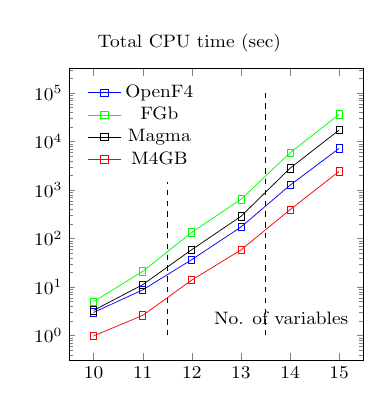
\begin{tikzpicture}[xscale=0.7, yscale=0.65]
      \begin{semilogyaxis}
        [ title={Total CPU time (sec)},%, for the case $m=n+1$.},
		xlabel={No. of variables},
        % ylabel={CPU time (sec)},
        x label style={at={(axis description
            cs:.9,0.1)},anchor=south}, legend pos=north west, legend
        style={draw=none,fill=none}, grid style=dashed, xscale = 0.78
        ] \addplot[color=blue,mark=square] coordinates{(10, 2.99)(11,
          8.73)(12, 36.76)(13, 172.49)(14, 1258)(15, 7225)};
				
		\addplot[color=green,mark=square]
        coordinates{(10,5)(11,21)(12,134)(13,642)(14,5850)(15,36361)};
		
		\addplot[color=black,mark=square]
        coordinates{(10,3.29)(11,11.172)(12,59.08)(13,286.4)(14,2810.75)(15,17265.5)};
		
		\addplot[color=red,mark=square] coordinates{(10, 0.98)(11,
          2.6)(12, 13.92)(13,58.18)(14, 393.19)(15, 2424)};
		
		\addplot +[mark=none,color=black, style=dashed] coordinates
        {(11.5, 1) (11.5, 1500)};
        % \node[anchor={north west},rotate=270] at (axis cs:
        % 11.5,1500) { DoR 7 };
        % \node[anchor={south west},rotate=270] at (axis cs:
        % 11.5,1500) { DoR 8 };
		
		\addplot +[mark=none,color=black, style=dashed] coordinates
        {(13.5, 1) (13.5, 100000)};
        % \node[anchor={north west},rotate=270] at (axis cs:
        % 13.5,100000) { DoR 8 };
        % \node[anchor={south west},rotate=270] at (axis cs:
        % 13.5,100000) { DoR 9 };
		
		\legend{OpenF4, FGb, Magma, M4GB}
      \end{semilogyaxis}
    \end{tikzpicture}
    \hspace{10mm}
    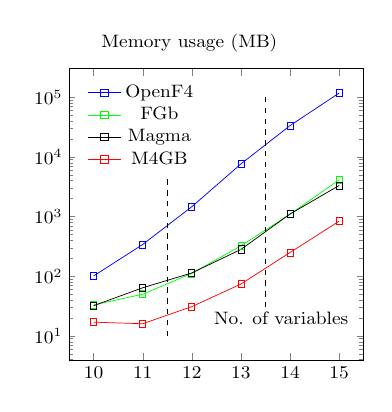
\begin{tikzpicture}[xscale=0.7, yscale=0.65]
      \begin{semilogyaxis}
        [ title={Memory usage (MB)},% for the case $m=n+1$.},
		xlabel={No. of variables}, x label style={at={(axis
            description cs:.9,0.1)},anchor=south},
        % ylabel={Memory (Mbytes)},
		legend pos=north west, legend style={draw=none,fill=none},
        grid style=dashed, xscale = 0.78 ]
        \addplot[color=blue,mark=square]
        coordinates{(10,101)(11,341)(12,1463)(13,7622)(14,33460)(15,117396)};
				
		\addplot[color=green,mark=square]
        coordinates{(10,33)(11,50)(12,112)(13,323)(14,1098)(15,4118)};
		
		\addplot[color=black,mark=square]
        coordinates{(10,32.09)(11,64.12)(12,113.59)(13,281.53)(14,1104)(15,3320)};
		
		\addplot[color=red,mark=square]
        coordinates{(10,17)(11,16)(12,31)(13,74)(14,250)(15,837)};
		
		\addplot +[mark=none,color=black, style=dashed] coordinates
        {(11.5, 10) (11.5, 5000)};
        % \node[anchor={north west},rotate=270] at (axis cs:
        % 11.5,7500) { DoR 7 };
        % \node[anchor={south west},rotate=270] at (axis cs:
        % 11.5,7500) { DoR 8 };
		
		\addplot +[mark=none,color=black, style=dashed] coordinates
        {(13.5, 30) (13.5, 100000)};
        % \node[anchor={north west},rotate=270] at (axis cs:
        % 13.5,180000) { DoR 8 };
        % \node[anchor={south west},rotate=270] at (axis cs:
        % 13.5,180000) { DoR 9 };
		
		\legend{OpenF4, FGb, Magma, M4GB}
      \end{semilogyaxis}
    \end{tikzpicture}
  \end{frame}
\end{section} %Performance Comparison

\begin{section}{Solving MQ Challenges}

  \begin{frame}{Solved MQ Challenges}
    \begin{table}
      \center
      \begin{tabular}{|c|c|c|c|}
        \cline{2-4}
        \multicolumn{1}{c|}{} & $\FField{2}$ & $\FField{2^8}$ & $\FField{31}$\\
        \hline
        \multirow{2}{*}{$m = 2n$} & \Large{I} &  \Large{II} & \Large{III} \\
        \cline{2-4}
        & $n \geq 55$ & $n \geq 35$ & $n \geq 34$\\
        \hline
        \hline
        \multirow{2}{*}{$m \approx 2/3 n$} & \Large{IV} & \color<2->{orange}{\Large{V}} & \color<2->{orange}{\Large{VI}} \\
        \cline{2-4}
        & $m \geq 55$ & $m \geq 16$ & $m \geq 16$\\
        \hline
      \end{tabular}
    \end{table}
  \end{frame}

  \begin{frame}{Solving Strategy}
    \begin{itemize}
    \item<2-> Hybrid approach
    \item<3-> Idea :
      \begin{enumerate}
      \item<4-> Randomly select
        $(a_1, \ldots, a_{n-m}) \in \FField{q}^{n-m}$
      \item<5-> Construct
        $$
        \tilde{F} = \{ f(x_1, \ldots, x_m, a_1, \ldots, a_{n-m}) :
        \forall f \in F \}
        $$
      \item<6-> Select small positive integer $k$ (e.g. $1$ or $2$)
      \item<7-> Generate $q^k$ subsystems
        $$
        \{ \tilde{F}(x_1, \ldots, x_{n-k}, v_1, \ldots, v_k) : (v_1, \ldots, v_k) \in \FField{q}^k\}
        $$
      \item<8-> Compute \Grobner basis of each subsystem
      \end{enumerate}
    \end{itemize}
  \end{frame}

  \begin{frame}{Summary of Solved Challenges}
    \begin{table}
      \begin{tabular}{|c|c|c|c|c|}
        \hline
        Type & $n/m$ & Machine Used & \# Node & Duration \\
        \hline
        \onslide<2->{V} & \onslide<2->{$24/16$} & \onslide<3->{A} & \onslide<3->{$1$} & \onslide<3->{$\approx 9.3$ hours}\\
        \onslide<2->{V} & \onslide<2->{$25/17$} & \onslide<4->{B} & \onslide<4->{$1$} & \onslide<4->{$\approx 46.33$ hours}\\
        \onslide<2->{V} & \onslide<2->{$27/18$} & \onslide<4->{B} & \onslide<4->{$2$} & \onslide<4->{$\approx 10.9$ days}\\
        \hline
        \hline
        \onslide<5->{VI} & \onslide<5->{$24/16$} & \onslide<6->{A} & \onslide<6->{$1$} & \onslide<6->{$\approx 1.2$ hours}\\
        \onslide<5->{VI} & \onslide<5->{$25/17$} & \onslide<7->{B} & \onslide<7->{$1$} & \onslide<7->{$\approx 9.87$ hours}\\
        \onslide<5->{VI} & \onslide<5->{$27/18$} & \onslide<7->{B} & \onslide<7->{$1$} & \onslide<7->{$\approx 31.48$ hours}\\
        \onslide<5->{VI} & \onslide<5->{$28/19$} & \onslide<7->{B} & \onslide<7->{$2$} & \onslide<7->{$\approx 7.61$ days}\\
        \hline
      \end{tabular}
    \end{table}
    \vspace{10mm}
    \begin{footnotesize}
        A) Intel(R) Core(TM) i7-2600K CPU @3.40GHz and 16GB RAM (Desktop)\\
        B) Intel(R) Xeon(R) CPU E5-2650 v3 @ 2.30GHz and 128GB RAM (NUMA)
    \end{footnotesize}
  \end{frame}

\end{section} %Solving MQ Challenges


\begin{frame}
  \center{\url{https://github.com/cr-marcstevens/m4gb}}
\end{frame}


\begin{frame}
  \center{Question ?}
\end{frame}


\end{document}
